\documentclass[12pt]{report}
% chktex-file 44
% chktex-file 40

\usepackage{algorithm2e} \usepackage{amsmath} \usepackage{amssymb} \usepackage{fancyref}
\usepackage{indentfirst} \setlength\parindent{24pt}
\usepackage{float} \usepackage[margin=1in]{geometry} \usepackage{graphicx} \usepackage{hyperref}
\usepackage{setspace} \usepackage[nottoc,numbib]{tocbibind}
\usepackage[backend=biber,citestyle=numeric-comp]{biblatex}
\usepackage{collcell} \newcommand{\fwcell}[1]{\makebox[\arraystretch\normalbaselineskip]{$#1$}}
\usepackage{tcolorbox} \tcbuselibrary{theorems}
\usepackage{amsthm}

\usepackage{graphicx} \graphicspath{{./images/}}

\tolerance=1
\emergencystretch=\maxdimen{}
\hyphenpenalty=10000
\hbadness=10000

\newtcbtheorem[number within=section]{defbox}{Definition}%
{colback=lightgray!5,colframe=lightgray!35!black,
  fonttitle=\bfseries}{th}

\newtcbtheorem[number within=section]{thmbox}{Theorem}%
{colback=lightgray!5,colframe=lightgray!35!black,
  fonttitle=\bfseries}{th}

\addbibresource{references.bib}

\title{A Novel Approach to Computing Magic Squares Using Group Theory} \author{Nathan Keough \\
  \href{mailto:nathan.keough@my.maryvillecollege.edu}{nathan.keough@my.maryvillecollege.edu} }
\date{\today}

\begin{document}

\setcounter{chapter}{-1}

% \renewcommand{\chaptername}{}
% \renewcommand{\thechapter}{}

\pagenumbering{roman}

\maketitle
\pagebreak

\singlespacing{}
\tableofcontents{}
\pagebreak

\doublespacing{}
\pagenumbering{arabic}

\begin{abstract}
  \par This paper introduces a novel algorithm for computing magic squares, exploiting
  group theory concepts such as permutation representation, group operations, and group actions to
  encode symmetries. By defining the group operation as composition, the set as a subset of the
  group of magic squares in a specific order, we may systematically explore the permutations of the
  group and extrapolate information about the magic squares to generate new magic squares not in
  the originating set. This vastly reduces computation times for enumerating the solutions to magic
  squares, while also encoding the symmetries in a manner that is easier to analyze
  programmatically. Overall, this study reveals the profound connection between magic squares and
  group theory, offering promising avenues for symmetry-driven algorithms and applications in
  combinatorial mathematics.
\end{abstract} \pagebreak

\chapter{Introduction}

\begin{figure}[h!]
  \begin{align*}
    \quad \renewcommand{\arraystretch}{2}
    \begin{tabular}{|
      *{3}{>{\collectcell\fwcell}c<{\endcollectcell} |} }
      \hline 2 & 9 & 4 \\
      \hline 7 & 5 & 3 \\
      \hline 6 & 1 & 8 \\
      \hline
    \end{tabular}
  \end{align*}
  \caption{Magic square.}\label{fig:square}
\end{figure}

\par The secrets behind magic squares have eluded mathematicians for millennia. The magic square
problem itself is believed to have originated in China around 2200 BCE with the introduction of
what are now known as “Lo-Shu” magic squares. These magic squares are defined as $3\times3$ grids
with the numbers $1$ through $9$ arranged such that the sums of all the rows, columns, and
diagonals are the same. Note in Fig.~\ref{fig:square} that the rows, columns, and diagonals each
add to $15$.

\par This property is what makes a square ``magic,'' lending a connotation of power that is
respected by many ancient cultures. In many ways, magic squares have held a mythical reputation in
culture due to their unique properties. As mathematics evolved, so did the study of magic squares
worldwide, later appearing in India, The Middle East, and Latin Europe. Each rendition of the magic
square problem brings with it new questions in mathematics. The number of solutions to the Lo-Shu
magic square problem is well known. However, The number of solutions to other kinds of squares
remains a great mystery, especially as the size of the square grows.

\par There is only one unique solution for the Lo-Shu Square, pictured in Fig.~\ref{fig:square}.
There are extensions to the magic square problem, with variants having larger side lengths (order),
different ``magic'' requirements, or different kinds of element values. For order four, there are
$880$ unique solutions. For order five, there are $275,305,224$ unique solutions. However, the
number of exact unique solutions for order six remains unknown. The number of unique solutions for
each order exhibits a kind of exponential growth, and their values have been of interest to
mathematicians and hobbyists since the puzzle's inception.

\par Today, magic squares hold less of a mythical and powerful cultural reputation. Mathematics, at
this point in history, has been able to deduce new and creative uses for magic squares in various
different fields, especially physics. In 2021, scientists found a connection between electrostatic
potentials and magic squares of the $5^{th}$ and $6^{th}$ order [CITE]. Similarly, magic squares of
the $6^{th}$ order have been associated with the Weak Force in physics [CITE]. Outside of physics,
there are also uses for magic squares in image encryption, specifically, using large squares as
chaos maps in chaos-based encryption schemes [CITE]. For these reasons and many others, the
continual study of magic squares carries with it the possibility of new breakthroughs in applied
mathematics.

\par Although there are many kinds of magic squares, we will only interest ourselves in ``normal''
magic squares, which have two main requirements: $(1)$ The square must be filled with the integers
from $1$ to $n^2$ inclusive, where $n$ is the order of the magic square, and $(2)$ the sums of the
main columns, rows, and diagonals must equal the same integer. This integer $S$ is called the
``magic sum'' and is calculated by $nS = \frac{n^2(n^{2}+1)}{2}$ with the right-hand side equating
to the sum of the first $n^2$ positive integers, and the left-hand side equal to the magic sum
multiplied by a factor $n$, the order of the square. Dividing by this factor on both sides
satisfies this equation for the magic sum. The number of rows, columns, and diagonals is equal to
$2n+2$ with $n$ being the order of the square. This is considered the number of ``constraint
vectors'' of a magic square.

\begin{figure}[h!]
  \begin{align*}
    \quad \renewcommand{\arraystretch}{2}
    \begin{tabular}{|
      *{3}{>{\collectcell\fwcell}c<{\endcollectcell} |} }
      \hline 2 & 9 & 4 \\
      \hline 7 & 5 & 3 \\
      \hline 6 & 1 & 8 \\
      \hline
    \end{tabular}
    \quad \renewcommand{\arraystretch}{2}
    \equiv
    \quad \renewcommand{\arraystretch}{2}
    \begin{tabular}{|
      *{3}{>{\collectcell\fwcell}c<{\endcollectcell} |} }
      \hline 6 & 7 & 2 \\
      \hline 1 & 5 & 9 \\
      \hline 8 & 3 & 4 \\
      \hline
    \end{tabular}
  \end{align*}
  \caption{The magic squares are equivalent.}\label{fig:unique}
\end{figure}

\par We are also only interested in studying ``unique'' magic squares. By this, we mean magic
squares that are unique up to rotations and reflections. An example of this is taking a magic
square $A$ and rotating it $90^{\circ }$ or reflecting it about the y-axis any number of times. The
resulting square will always be considered equivalent to $A$. There may also be times when we refer
to a ``positionally distinct'' magic square. In this case, reflections or rotations of a magic
square $A$, results in a ``different'' square $B$. Neither of these definitions affect the validity
of magic squares; they only affect how we count them. Fig.~\ref{fig:unique} accurately represents
two magic squares that we would consider to be the ``same'' square.

\par To help us compute magic squares, we have implemented a custom Computational Algebra System
(CAS) written in the Rust Programming Language. This system allows us to construct and manipulate
square data to find magic squares. Once we have magic squares, we may do additional processing on
them to learn more about their structures. The system is geared for high performance and thus
implements some of the best known strategies for working with magic square structures, both
mathematically and programmatically.

\section{Permutations}

\par The main mechanism that we use for encoding a magic square and its properties comes from Group
and Number Theory. Specifically, we will study the permutations of magic squares. In the 1770s,
Joseph Louis Lagrange studied permutations of the roots of polynomial equations. This led to Galois
theory founded by Évariste Galois, which describes what is or is not possible with respect to
solving polynomial equations by radicals [CITE]. In modern mathematics, there are many similar
situations where studying permutations can help us understand a problem.

\par Roughly speaking, magic squares may be represented as permutations of $n^2$ objects. By the
definition of a normal magic square, these are the positive integers (mod $n^2$). The dimension
need not matter since the coordinates of elements in a two-dimensional, row-major grid square may
be mapped to a one-dimensional sequence, which is a bijection. The square, laid out as a
one-dimensional sequence, represents the sequence of integers as a permutation. There are total of
$n^{2}$! permutations of a square, that is $n^2$ factorial permutations, $n$ being the order of the
square. The permutations of squares represent the different possible configurations of integers in
the square, many of them meeting the requirements to be considered magic squares.

\par We believe that by studying different permutations of squares, including those that are magic,
we may be able to describe various kinds of symmetry related to magic squares of specific orders.
Treating individual squares as permutations and vice-versa allows us to make use of the properties
relating to permutations in general, meaning we can perform unique transformations or actions on
them using methods originating from group theory. Additionally, we may define other mathematical
properties that allow us to better describe magic squares and their associated symmetries that go
beyond simple row and column transposition.

\section{Enumeration}

\par In our investigation into the inner structures and symmetries of magic squares, we may find it
useful to enumerate the magic squares, i.e.\ exhaustively listing and analyzing every magic square
of a specific order. By hand, this is futile, but with high performance programming, we can do this
very easily for certain orders and with certain algorithms. Listing magic squares in this way, as
we will see, is useful and allows us to generalize certain properties of magic squares, potentially
also for higher orders.

\par Recall that the number of permutations of $n$ objects is $n$!. We can actually exploit this
fact to implement an element of ordering for magic squares. There exists a natural ordering from
$S_n$, the group of all permutations on $n$ elements, to $\mathbb{Z}^{*}_{n!-1}$  in the
factor-adic number system, (*) meaning non-negative. This number system, also known as the
factorial number system, is a mixed radix adapted for combinatorial systems. In this system, we can
express the permutations of $n$ objects in lexicographical order, that is naturally from $0$ to
$n!-1$ as a bijection. Using the factor-adic number system's properties we can treat magic squares
(or any grid square) as a permutation, and map that permutation uniquely to an integer. More
generally, this concept is called a Lehmer Encoding of a permutation on $n$ integers [CITE]. This
not only simplifies our intuition of what a unique magic square looks like, but also improves the
performance of a magic square computation in some cases, specifically, the cost of copying integers
over whole arrays and storing magic squares in memory.

\par It should be noted that the indices of magic squares in their ordered set do not follow an
easily identifiable pattern. Perhaps there is a pattern, but we have no way of identifying it based
on our current assumptions of magic squares. In any case, analyzing the frequency of magic squares
in their ordered set has not so far proved to be helpful. Exhaustive enumeration of magic squares
is presumed to be an NP-Hard problem, making it suitable for certain cryptographic applications.
However, it is at least NP;\@ the NP-completeness and classification of the magic square problem is
formally unknown. The complexity of predicting magic squares is unknown, yet, there do exist
applications in artificial intelligence for predicting and classifying magic squares [CITE].

\chapter{Permutation Groups}

\section{Introduction}

\par The set of magic square solutions falls under the definition of a permutation group.
Generally, there are many kinds of permutation groups. For example, Sn is considered a permutation
group, but as a whole, it is typically considered a representation of the symmetric group.

\singlespacing{}
\begin{defbox}{}{defperm}
  Let $S$ be a set with $n$ elements. Let $\varGamma\left(S\right)$ represent the set of
  permutations of $S$. Let $\left(\varGamma\left(S\right), \circ \right)$ be the algebraic
  structure
  such that $\circ$ denotes the composition of mappings. Then, $\left(\varGamma\left(S\right),
    \circ
    \right)$ is the symmetric group on S, also known as $S_n$.
\end{defbox}
\doublespacing{}

\par Additionally, a permutation group may be considered a subgroup of the symmetric group on $S$,
a set of $n$ integers.

\singlespacing{}
\begin{thmbox}{}{thmperm}
  \textbf{A Permutation Group is a Subgroup of The Symmetric Group}
  \begin{proof}[Proof:]
    Recall that $\left(\varGamma\left(S\right), \circ \right)$ is the symmetric group on $S$ of $n$
    elements ($S_n$). Let $\left(H,\circ\right)$ be a set of permutations of $S$ forming a group
    under
    $\circ$. Following the definition of a subgroup, $\left(H,\circ\right)$ is a subgroup of
    $\left(\varGamma\left(S\right), \circ \right)$,\\ $\therefore$ a permutation group is a
    subgroup of
    $S_n$.
  \end{proof}
\end{thmbox}
\doublespacing{}

\par A set of magic squares may also be considered a permutation group. The group operation, in
this case, is multiplication. This is different from the typical arithmetic operation. Rather, it
could be called “composition” since the behavior of multiplication on a permutation resembles
function composition. We may think of permutations as functions that bijectively map a set to
itself. The product of two functions, $\pi\cdot\sigma$ is the function mapping any element $x$ in
the set to $\pi\left(\sigma\left(x\right)\right)$. Generally, the operation is defined for left
multiplication, but since these are permutation representations (and to simplify expressions in our
code) we will use right multiplication. In other words ``$\pi$ is permuted by $\sigma$'' or ``$\pi$
is acted on by $\sigma$''.

\par It follows that a permutation composed with a permutation results in another permutation.
Notably, we can define a function $g$ to be the group operation of composition, and $X$ to be a
permutation group. Then $g:X\rightarrow X$ denotes that g is a function mapping any element in $X$
back to another element in $X$ which is a group endomorphism. Any composition of permutations
results in a permutation.

\singlespacing{}
\begin{thmbox}{}{thmcomp}
  \textbf{Composite of a Permutation is a Permutation}
  \begin{proof}[Proof:]
    Let $\pi,\sigma$ be permutations of the set $S$, and $\pi\circ\sigma$ denotes the composite of
    the permutations. Recall that a permutation of $S$ is a bijection, and that composition of
    bijections is a bijection. Their domain and codomains are coincident,\\ $\therefore
      \pi\circ\sigma$
    must also be a permutation of $S$.
  \end{proof}
\end{thmbox}
\doublespacing{}

\par Generally, we may study how magic squares behave under multiplication. Magic squares, being
permutations in $S_{n^2}$, exhibit group properties. However, we may not describe a set of magic
squares as a group due to the absence of the identity permutation or an identity magic square,
inverses, and closure. Rather, we may treat a set $K$ of magic squares as a set of generators for
some group. With these generators, we may force closure of the permutation group under composition,
thus enabling further group exploration. It is important to note, now, that forcing closure does
not always preserve the magic property of the permutations, as in the original set $K$ \hyphen{}
this group simply contains the elements of $K$, which is a set of known magic squares. The same
definition can be applied for the set containing all magic squares of order $n$. This set, which we
call $M_n$, denotes a permutation group closed under composition, in which all permutations
representing magic squares of order $n$ are members.

\par Due to the properties imposed on $M_n$, we can treat it as a permutation group, though we
generally don't know much about this group, aside from its properties. Taking a more computational
route normally involves already knowing some information about the group's generators or internal
structure. With these, far more can be learned and analysis of the group then is trivially
dependent on computation time. For magic squares, this is not the case since not much is known
about how the internal structures and generating subsets generalize for larger order squares. The
route we are left with is to use iterative brute force methods to find the generators of $M_n$ so
that we may perform further analyses.

\chapter{Group Actions}

\section{Introduction}

\par A rational way to understand a complicated or obscure group is to let it act on something. The
concept of a group action in the context of group theory defines a set of functions that act on a
specific group. These functions may also be considered transformations of the group. The functions
applied to elements in the group produce permutations of the group and define the kind of
transformations that exist between elements of the group.

\singlespacing{}
\begin{defbox}{}{defaction}
  Let $G$ be a group and let $S$ be a set. Define an action on $S$ by $G$ to be a homomorphism
  $\varphi:G\rightarrow Sym\left(S\right)$
\end{defbox}
\doublespacing{}

A simple example would be the set of transformations of a Rubix Cube. The set of transformations or
actions of a Rubix Cube may be described by the possible moves a player may take to change the cube
i.e.\ rotating specific segments in different directions on various axes. These group actions serve
as a basis for the type of configurations we can produce on a Rubix Cube. More generally, they
describe the kinds of permutations that can exist in a group, given a set $S$ of permutations and
group $G$ that acts on it via composition.

\section{Dihedral Groups}

\par We apply the concept of a group action heavily in our code. Specifically, the idea of a group
acting on a set defines how we know if a magic square is unique or not. Although the actual square
data is flat, we may imagine the magic square in its normal grid square arrangement. We define a
unique magic square as a magic square unique up to rotations and reflections. This means that the
action of rotating, reflecting, or any combination of rotations and reflections will not result in
a new magic square being enumerated. It should be noted that these transformations are
magic-preserving since they do not alter the distances between consecutive elements in the grid.
Only one magic square from the set of its rotations and reflections is counted; the rest are
considered the ``same'' square.

\par The set of structure-preserving transformations of a square (or any regular polygon) actually
has its own name: the dihedral group denoted $D_n$. A regular polygon has $2n$ symmetries \hyphen{}
$n$ rotational and $n$ reflection symmetries. We may also call it $D_{2n}$ due to this fact. In any
case, $D_8$ is the group of rigid symmetries of a square. This dihedral group encodes all of the
orientations of a unique magic square. However, magic squares contain more than four elements, thus
the rotations and reflections of magic squares are merely congruent to $D_8$.

\begin{figure}[H]
  \begin{align*}
    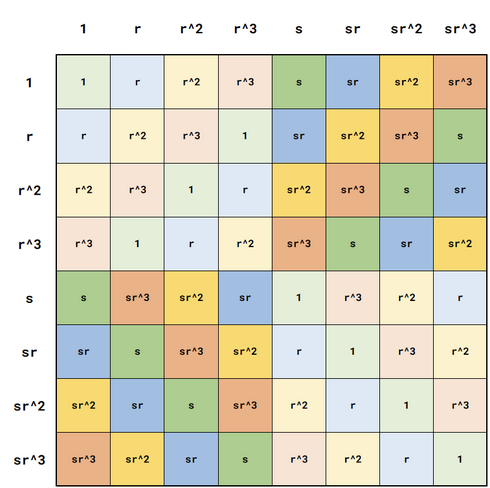
\includegraphics[scale=0.6]{cayleytable.png}
  \end{align*}
  \caption{Cayley Table of $D_8$}\label{fig:cayley}
\end{figure}

\par Computationally, we can select a unique element from the square's dihedral group consistently
by selecting the first element from the Cayley table of transformations. Alternatively, we can
generate the full set of the dihedral group. This table, shown in Fig.~\ref{fig:cayley}, represents
the transformations of the dihedral group D generated by $<r,s\vert
  r^4=s^2={\left(sr\right)}^2=1>$. We treat the table like a set and filter another set containing
various arbitrary magic squares such that the resulting set only contains unique elements. This is
useful for brute-force algorithms where we may not have total control over element uniqueness in a
set. The same applies for certain constructive algorithms, but still, we ensure that we do not
duplicate magic squares in our sets, resulting in better analysis and more efficient runtimes.

\section{Group Actions on Magic Squares}

\par In the same manner that the dihedral group applied to the permutation of a square results in
the same square, the dihedral group applied to a magic square always results in a magic square.
This property represents a symmetry of a magic square. Specifically, it represents the rotational
and reflective symmetry of an arbitrary magic square. Based on this, the application of group
actions on sets presents itself as a potential medium for representing group symmetry in the magic
square permutation group.

\par If we assume that the full set of magic squares is known, the group actions of the set would
be the full set of transformations between magic squares in the set. One thing we are interested in
is if these actions can tell us something new about the set that we didn't know before. Are there
additional magic-preserving sets of permutations, like those from the dihedral group? How many
symmetries exist for magic squares of a specific order? The answers to these questions may reveal
new patterns, lead to more efficient methods, or allow us to use smaller search-spaces for larger
orders.

\par Computationally, we can produce the transformation between two magic squares, $\pi$ and
$\sigma$, by factoring out the permutation $\alpha$ that acts on $\pi$ to produce $\sigma$. The
factorization of permutations is a well known problem and is computed by inverting part of the
original composition:

\begin{align*}
  00
\end{align*}

\chapter{Solving Magic Squares}

\section{Introduction}

\section{Current Method}

\section{New Method}

\chapter{Analysis}

\section{Introduction}

\section{Computational Analysis}

\section{Generating Sets}

\section{Magic-Preserving Group}

\chapter{Conclusions}

\section{Introduction}

\section{Alternative Methods}

\section{Generalizations}

\section{Open Questions}

\nocite{*}
\printbibliography{}

\end{document}